\documentclass[10pt]{article}
\usepackage[utf8]{inputenc}
\usepackage{amsmath}
\usepackage{amssymb}
\usepackage{graphicx}
\usepackage{hyperref}
\title{openAPE}
\author{Stephan Unfried}
\date{\today} 
\begin{document}
\maketitle
\newpage
\tableofcontents
\newpage
\section{Introduction}
\section{project structure}
\subsection{Modules}
The project consists of tree parts, represented in tree maven modules. For details of the associations see figure \ref{fig:moduleuml}.
\begin{figure}[b]
\centering
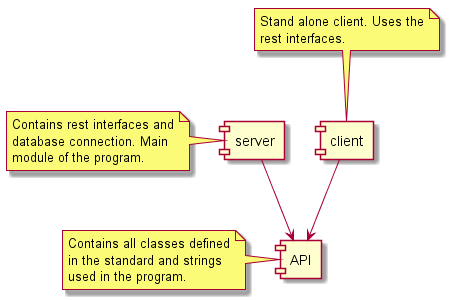
\includegraphics[width=1\textwidth]{uml/modulesuml.png}
\caption{module diagram.}
\label{fig:moduleuml}
\end{figure}
\subsection{API}
API contains classes and class structure used by the application server and clients who want to communicate with it. The classes 
\begin{figure}[b]
\centering
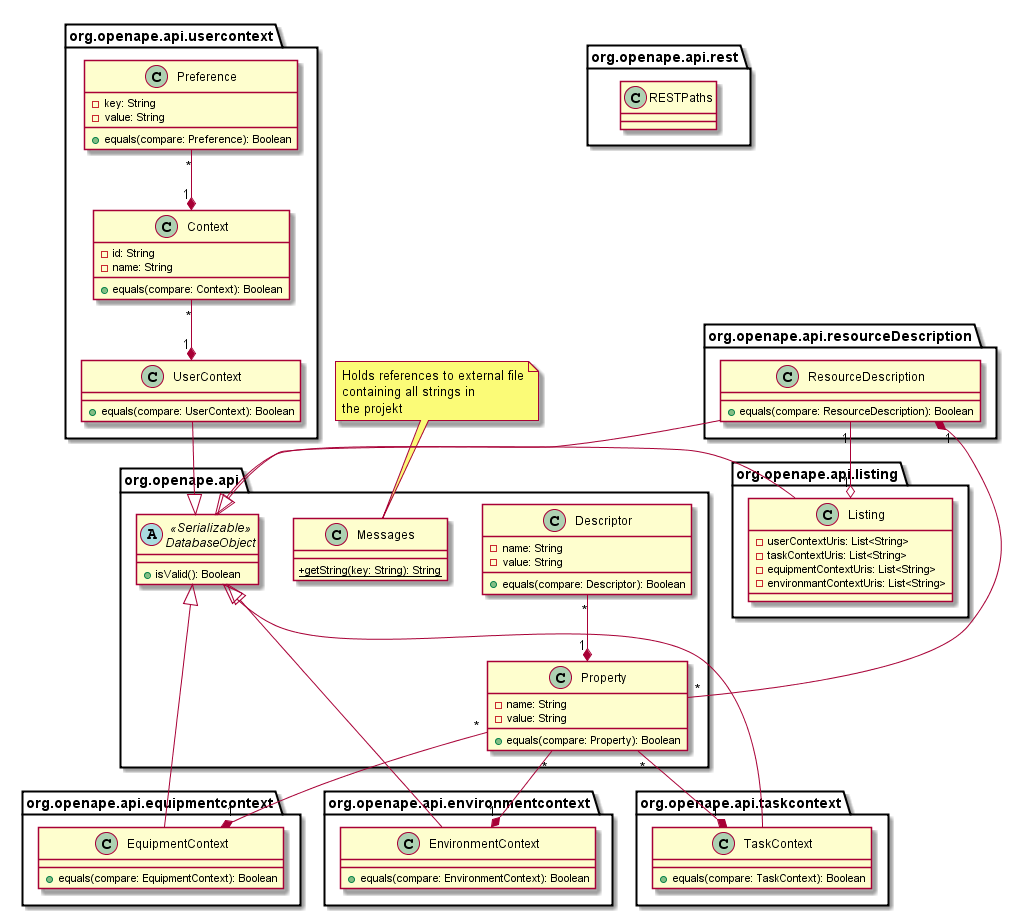
\includegraphics[width=1\textwidth]{uml/apiuml.png}
\caption{API module structure diagram.}
\end{figure}
\subsection{API}
\section{Get started with the project}
\section{Set up MonoDB}
\section{Set up tomcat server}
\end{document}
